% lmderRLD.tex
% $Author$ $Date$

\section{Levenberg--Marquardt searches for \rpo s}
\label{sec:lmderRLD}

To find \rpo s of the \KS\ flow, we use multiple shooting and
the Levenberg--Marquardt (LM) algorithm implemented in the routine
{\tt lmder} from the MINPACK software package\rf{minpack}.

In order to find periodic orbits, a system of nonlinear
algebraic equations needs to be solved.  For flows, this
system is underdetermined, so, traditionally, it is augmented
with a constraint that restricts the search space to be
transversal to the flow (otherwise, most of the popular
solvers of systems of nonlinear algebraic equations, e.g.
those based on Newton's method, cannot be used). When
detecting \rpo s, a constraint is added for each continuous
symmetry of the flow.  For example, when detecting relative
periodic orbits in the complex Ginzburg Landau equation,
L{\'o}pez {\etal}\rf{lop05rel} introduce three additional
constraints.

Our approach differs from those used previously in that we do
not introduce the constraints.  Being an optimization solver,
the LM algorithm has no problem with solving an
underdetermined system of equations, and, even though {\tt
lmder} explicitly restricts the number of equations to be not
smaller than the number of variables, the additional
equations can be set identically equal to
zero\rf{Crofts07thesis}.  In fact, there is numerical
evidence that, when implemented with additional constraints,
the solver usually takes more steps to converge from the same
seed, or fails to converge at all\rf{Crofts07thesis}. In what
follows we give a detailed description of the algorithm and
the search strategy which we have used to find a large number
of \rpo s defined in \refeq{KSrpos} and pre-periodic orbits
defined in \refeq{KSpos}.

When searching for \rpo s of truncated \KS\ equation
\refeq{eq:KS}, we need to solve the system of $N-2$ equations
\beq
  {\bf g}(\shift)f^\period{}(a) - a = 0\,,
\ee{eq:system}
with $N$ unknowns $(a, \period{}, \shift)$, where $f^t$
is the flow map of the \KSe.  In the case of pre-periodic orbits, the system has
the form
\beq
  -{\bf g}(-\shift)[f^\period{}(a)]^\ast - a = 0\,,
\ee{eq:systemppos}
(see \refeq{KSposFour}).

We have tried two different implementations of the multiple shooting.
The emphasis was on the simplicity of the implementations, so, even
though both implementations worked equally well, each of them had
its own minor drawbacks.

In the first implementation, we fix the total number of steps within
each shooting stage and change the numerical integrator step size
$h$ in order to adjust the total integration time to a desired value
$\period{}$.

Let $(\hat{a}, \hat{\period{}}, \hat{\shift})$ be the starting guess for a \rpo\
obtained through a close return within a chaotic attractor (see below).
We require that the initial integration step size
does not exceed $h_0$, so we round off the
number of integration steps to $n = \lceil \hat{\period{}}/h_0\rceil$, where
$\lceil x \rceil$ denotes the nearest integer larger than $x$.

The integration step size is equal to $h = \period{}/n$. With the
number of shooting stages equal to $m$, the system in
\refeq{eq:system} is rewritten as follows
\begin{eqnarray}\label{eq:MultShoot}
 F^{(1)}&\!=\!& f^\tau(a^{(1)}) - a^{(2)} = 0\,,\nonumber\\
 F^{(2)}&\!=\!& f^\tau(a^{(2)}) - a^{(3)} = 0\,,\nonumber\\
 && \cdots \\
 F^{(m-1)}&\!=\!& f^\tau(a^{(m-1)}) - a^{(m)} = 0\,,\nonumber\\
 F^{(m)}&\!=\!& {\bf g}(\shift)f^{\tau'}(a^{(m)}) - a^{(1)} = 0\,,\nonumber
\end{eqnarray}
where $\tau = \lfloor n/m \rfloor h$ ($\lfloor x \rfloor$ is the nearest
integer smaller than $x$),
$\tau' = nh - (m-1)\tau$, and $a^{(j)} = f^{(j-1)\tau}(a)$,
$j = 1, \ldots , m$.  For the detection of pre-periodic orbits, the last equation
in \refeq{eq:MultShoot} should be replaced with
\[
 F^{(m)} = -{\bf g}(-\shift)[f^{\tau'}(a^{(m)})]^\ast - a^{(1)} = 0\,.
\]
With the \jacobianM\ of \refeq{eq:MultShoot} written as
\beq
  J = \left(\begin{array}{ccc}\!\!
   \displaystyle \frac{\partial F^{(j)}}{\partial a^{(k)}} &
   \displaystyle \frac{\partial F^{(j)}}{\partial \period{}} &
   \displaystyle \frac{\partial F^{(j)}}{\partial \shift}\!\!
  \end{array}\right),\quad j,k = 1,\ldots,m\,,
\eeq
the partial derivatives with respect to $a^{(k)}$ can be calculated
using the solution of \refeq{eq:KStan} as described in
\refappe{sec:stability}.  The partial derivatives
with respect to $T$ are given by
\beq
  \frac{\partial F^{(j)}}{\partial \period{}} =
  \left\{\begin{array}{ll}
    \frac{\partial f^\tau(a^{(j)})}{\partial \tau}
    \frac{\partial \tau}{\partial T} = v(f^\tau(a^{(j)}))
    \lfloor n/m \rfloor/n\,, & j = 1,\ldots, m-1\\[.5ex]
    {\bf g}(\shift) v(f^{\tau'}(a^{(j)}))
    (1 - \frac{m-1}{n} \lfloor n/m \rfloor ), & j = m\,.
  \end{array}\right.
\eeq
Note that, even though $\partial f^t(a) /\partial t = v(f^t(a))$,
it should not be evaluated using \edit{the} equation for the vector field \edit{$v$}.
The reason is that, since the flow $f^t$ is approximated by a
numerical solution, the derivative of the numerical solution with
respect to the step size $h$ may differ from the vector field $v$,
especially for larger step sizes.  We evaluate the derivative by
a forward difference using numerical integration with step sizes
$h$ and $h + \delta$:
\beq
  \frac{\partial f^{jh}(a)}{\partial t} = \frac{1}{j\delta}
  \left[f^{j(h+\delta)}(a) - f^{jh}(a)\right],\quad j \in
  {\mathbb Z}^{+}
\eeq with $t = jh$ and $\delta = 10^{-7}$ for double precision
calculations. Partial derivatives $\partial F^{(j)}/\partial \shift$
are all equal to zero except for $j = m$, where it is given by
\beq
  \frac{\partial F^{(m)}}{\partial \shift} =
  \frac{d{\bf g}}{d\shift}f^{\tau'}(a^{(m)}) =
  \diag(i q_k e^{i q_k\, \shift} )f^{\tau'}(a^{(m)})\,.
\eeq

This \jacobianM\ is supplied to {\tt lmder}
augmented with two rows of zeros corresponding to the two identical
zeros augmenting \refeq{eq:MultShoot} in order to make the number of
equations formally equal to the number of variables,
as discussed above.

In the second implementation, we keep $h$ and $\tau$ fixed and vary
only $\tau' = \period{} - (m-1)\tau$.  In this case, we need to be
able to determine the numerical solution of \KSe\ not only at times
$t_j = jh, j = 1, 2, \ldots$, but at any intermediate time as well.
We do this by a cubic polynomial interpolation through points
$f^{t_j}(a)$ and $f^{t_{j+1}}(a)$ with slopes $v(f^{t_j}(a))$ and
$v(f^{t_{j+1}}(a))$.  The difference from the first implementation
is that partial derivatives $\partial F^{(j)}/\partial \period{}$
are zero for all $j = 1,\ldots,m-1$, except for
\beq
  \frac{\partial F^{(m)}}{\partial \period{}} =
  {\bf g}(\shift)v(f^{\tau'}(a^{(m)}))\,.
\eeq
which, for consistency, needs to be evaluated from the cubic
polynomial, not from the flow equation evaluated
at $f^{\tau'}(a^{(m)})$.

For detecting \rpo s of the \KS\ flow with $L = 22$, we used
$N = 32$, $h = 0.25$ (or $h_0 = 0.25$ within the first implementation),
and a number of shooting stages such that $\tau \approx 40.0$.
While both implementations were equally successful in detecting
periodic orbits of \KS\ flow, we found the second implementation more
convenient.


%%%%%%%%%%%%%%%%%%%%%%%%%%%%%%%%%%%%%%%%%%%%%%%%%%%%%%%%%%%%%%
\begin{figure}[t]
\begin{center}
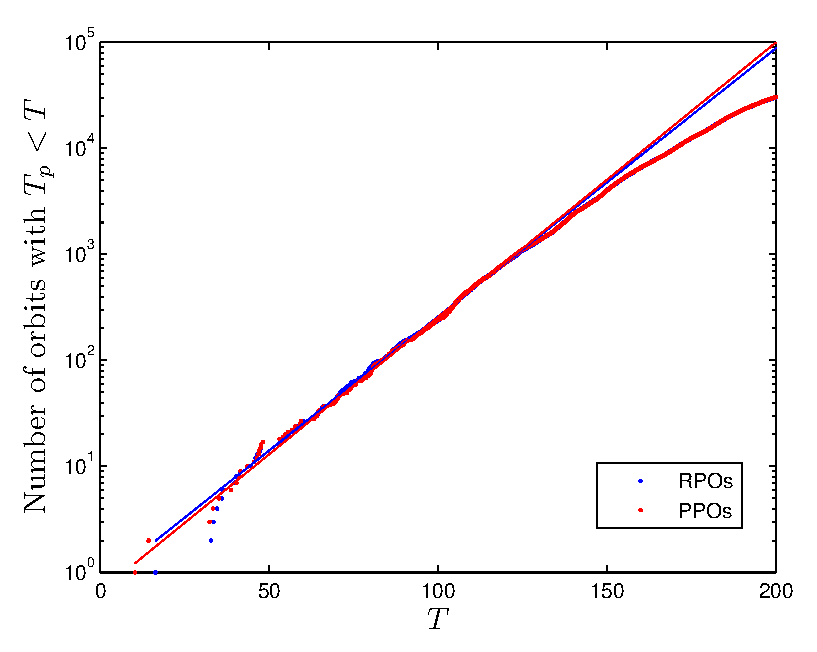
\includegraphics[width=0.9\textwidth, clip=true]{figs/ks22_Npos_30k.eps}
\end{center}
\caption{
Numbers of detected \rpo s (RPOs) and pre-periodic orbits (PPOs)
with periods smaller than $T$.  The lines indicate the linear fit
to the logarithm of the number of orbits as functions of $T$ in the
range $T \in [70, 120]$.
     } \label{fig:Npos}
\end{figure}
%%%%%%%%%%%%%%%%%%%%%%%%%%%%%%%%%%%%%%%%%%%%%%%%%%%%%%%%%%%%%%%%%%

The following search strategy was adopted: The search for
\rpo s with $\period{} \in [10, 200]$ was conducted within a
rectangular region containing the chaotic attractor.  To
generate a seed, a random point was selected within the
region and the flow \refeq{eq:KS} was integrated for a
transient time $t = 40$, sufficient for an orbit to settle on
the attractor at some point $\hat{a}$.  This point was taken
to be the seed location.  In order to find orbits with
different periods, the time interval $[10, 200]$ was
subdivided into windows of length 10, i.e. $[t_\mathrm{min},
t_\mathrm{max}]$, where $t_\mathrm{min} = 10j$ and
$t_\mathrm{max} = 10(j+1)$, with $j = 1, 2, \ldots, 19$.  To
determine the seed time $\hat{\period{}}$ and shift
$\hat{\shift}$, we located an approximate global minimum of
$\| {\bf g}(\shift)f^t(a) - a \|$ (or of $\| -{\bf
g}(-\shift)[f^t(a)]^\ast - a \|$ in the case of pre-periodic
orbits) as a function of $t \in [t_\mathrm{min},
t_\mathrm{max}]$ and $\shift \in (-L/2, L/2]$.  We did this
simply by finding the minimum value of the function on a grid
of points with resolution $h$ in time and $L/50$ in $\shift$.

Approximately equal numbers of seeds were generated for the
detection of \rpo s and pre-periodic orbits and within each
time window.  The hit rate, i.e. the fraction of seeds that
converged to \rpo s or pre-periodic orbits, varied from about
70\% for windows with $t_\mathrm{max} \leq 80$ to about 30\%
for windows with $t_\mathrm{min} \geq 160$.  The total number
of hits for \rpo s and pre-periodic orbits was over $10^6$
each.  Each newly found orbit was compared, after factoring
out the translation and reflection symmetries, to those already
detected.  As the search progressed, we found fewer and fewer
new orbits, with the numbers first saturating for smaller
period orbits.  At the end of the search we could find very
few new orbits with periods $T < 120$.  Thus we found over
30\,000 distinct prime \rpo s with $\shift > 0$ and over
30\,000 distinct prime pre-periodic orbits with $T < 200$.

In \reffig{fig:Npos} we show the numbers of detected \rpo s
and pre-periodic orbits with periods less than $T$.  It shows
that the numbers of \rpo s and pre-periodic orbits are
approx. equal and that they grow exponentially with
increasing $T$ up to $T \sim 130$, so that we are mostly
missing orbits with $T > 130$.  The straight line fits to the
logarithm of the numbers of orbits in the interval $T \in
[70, 120]$, represented by the lines in \reffig{fig:Npos},
indicate that the total numbers of \rpo s and pre-periodic
orbits with $T < 200$ could be over $10^5$ each.

To test the structural stability of the detected orbits and
their relevance to the full Kuramoto-Sivashinsky PDE, the
numerical accuracy was improved by increasing the number of
Fourier modes ($N = 64$) and reducing the step size ($h =
0.1$). Only a handful of orbits failed this higher-resolution
test. These orbits were not included in the list of the
60,000+ orbits detected.
